\documentclass[12pt]{article}
\usepackage{a4wide}
\usepackage{amsmath,amssymb}
\usepackage{bm}
\usepackage[colorlinks]{hyperref}
\usepackage{graphicx}

\usepackage{algorithm}
\usepackage{algorithmic}

\usepackage{float}
\usepackage{bbold}
\usepackage{comment}
\usepackage{mathtools}


%\usepackage{caption,refstyle}

% Package diagramme Processus de Production de la GS
\usepackage{tikz}
\usetikzlibrary{positioning, shadows}


\usepackage[french]{babel}
\usepackage[T1]{fontenc}
\usepackage{lmodern}

\DeclareUnicodeCharacter{2009}{\,} 
\usepackage[standard]{ntheorem}



\usepackage{tikz}
\usepackage{graphicx}
\usetikzlibrary{positioning, arrows.meta}
\usepackage{amsmath}



\begin{document}

\begin{titlepage}
\title{}
\author{Congo Job
\\ Stage Master 2 \\
 IRMA, Université de Strasbourg, France}
\date{ }

\begin{figure}[b!]
\centering
\vfill
\includegraphics[scale=0.16]{Images/logo-unistra.pdf}
\hspace{0.5 cm}
\includegraphics[scale=0.16]{Images/logo-Fonderie.pdf}
\hspace{0.5 cm}
\includegraphics[scale=0.16]{Images/logoCSMI.pdf}
\end{figure}
\end{titlepage}


\maketitle
\thispagestyle{empty}


\newpage

\tableofcontents

\newpage

% \section{Présentation de l'entreprise : Fonderie de Niederbronn}
\section{Introduction}



\subsection{Présentation de l'entreprise : Fonderie de Niederbronn}

%---- presenter la Fonderie,...

La Fonderie de Niederbronn, fondée en 1769, est un partenaire clé dans la production de pièces 
en fonte. Grâce à son expérience et son savoir-faire, l'entreprise produit des pièces en fonte 
à graphite lamellaire (GJL) et à graphite sphéroïdal (GJS) pour une clientèle industrielle variée,
aussi bien en France qu'à l'international. L’usine est située au Nord-Est de la France 
à Niederbronn près de Strasbourg.



\subsection*{Capacités et Installations de Production}
\textbf{Moyens de Fusion:}
\begin{itemize}
    \item 2 fours Junker 5T d'une puissance de 4MW.
\end{itemize}

\textbf{Lignes de Moulage:}
\begin{itemize}
    \item \textbf{DISAMATIC 270} : Coulée automatique verticale pour des pièces jusqu'à 950 x 700 mm et un poids maximum de 40 kg.
    \item \textbf{HWS} : Coulée automatique horizontale pour des pièces de dimensions jusqu'à 1600 x 1400 mm et un poids maximum de 600 kg.
\end{itemize}

\textbf{Moyens de Noyautage:}
\begin{itemize}
    \item 5 machines à noyer avec une capacité de production allant de 1 à 100 litres et des noyaux jusqu'à 300 kg.
\end{itemize}

\textbf{Moyens de Peinture:}
\begin{itemize}
    \item 2 lignes de peinture liquide pouvant traiter des pièces jusqu'à 500 kg. Peintures disponibles : primaire d'accrochage, peinture résistante aux brouillards salins de 300h, haute température (600°C).
\end{itemize}

\textbf{Moyens d'Usinage:}
\begin{itemize}
    \item Tours et centres d'usinage CNC avec des capacités variées pour des pièces de grandes dimensions (jusqu'à 1200 x 1000 x 600 mm).
\end{itemize}

\subsection*{Contrôle Qualité}
La Fonderie de Niederbronn attache une grande importance à la qualité de ses produits, mise en œuvre à travers divers contrôles :
\begin{itemize}
    \item \textbf{Dimensionnel:} Utilisation de bras FARO et scan 3D.
    \item \textbf{Non Destructif:} Banc de magnétoscopie et contrôle par ultrasons.
    \item \textbf{Caractéristiques Mécaniques:} Traction, contrôle de dureté, résilience.
    \item \textbf{Métallurgiques:} Spectrométrie et micrographie.
\end{itemize}

\subsection*{Secteurs d'Activité}
\sloppy
La Fonderie de Niederbronn sert plusieurs secteurs industriels et domestiques, 
en fournissant des pièces spécifiques adaptées aux besoins de chaque domaine.
\begin{itemize}
    \item \textbf{Usage Industriel :} Le Machinisme Agricole, les Machines du BTP, les Pièces Hydrauliques,...
    \item \textbf{Usage Domestique :} Les Corps de Chaudière et Radiateurs, les Poêles et Inserts de Cheminée,...
\end{itemize}

\subsection*{Chiffres Clés et Ressources Humaines}
\begin{itemize}
    \item \textbf{Nombre de Collaborateurs:} 170.
    \item \textbf{Capacité de Fusion:} 20 000 tonnes par an.
    \item \textbf{Chiffre d'Affaires:} 23 millions d'euros pour l'exercice 2023.
\end{itemize}


% - Mettre les 2 images fonderie vue de haut et une autre en vue de face.
\sloppy
Cette présentation met en lumière l'expertise, les capacités de production,
et l'engagement qualité de la Fonderie de Niederbronn, faisant d'elle un acteur 
incontournable dans le secteur de la fonderie.


\begin{figure}[H]
    \centering
    \vfill
    \includegraphics[scale=0.27]{Images/Fonderie_vue_de_bas.pdf}
    \hspace{0.5 cm}
    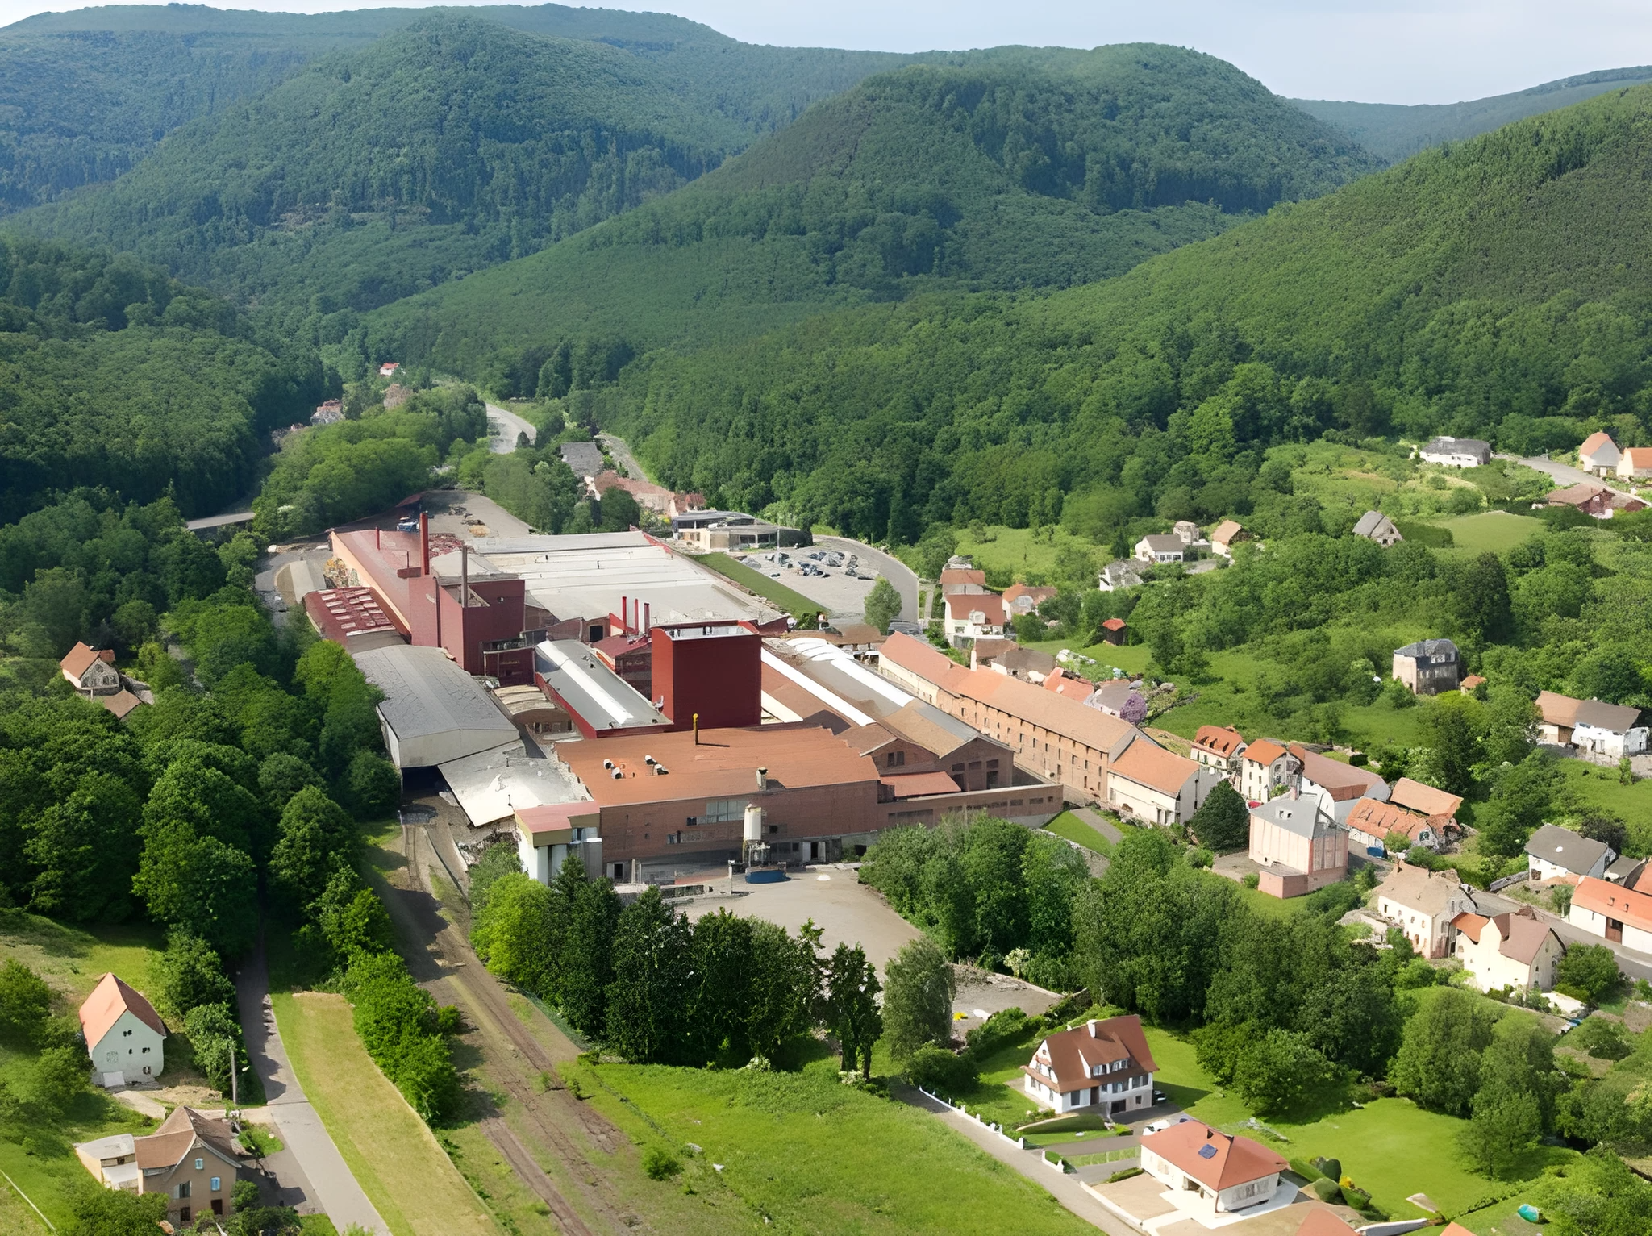
\includegraphics[scale=0.27]{Images/Fonderie_vue_de_haut.pdf}
    \caption{Vues extérieure et aérienne de la Fonderie de Niederbronn}
\end{figure}


\subsection{Contexte}

Dans ce stage, on cherche à optimiser la production de la fontes GS à chaque étape 
de son processus de productions. Voici un schema decrivant les differents etapes de 
la production de la fonte GS :




\begin{figure}[H]
    \centering
    \textbf{\Large \underline{Processus de Production de la fonte GS}}
    \vspace{0.5cm}

    \begin{tikzpicture}
        % Style des noeuds
        \tikzstyle{process} = [rectangle, rounded corners, minimum width=3.5cm, minimum height=1cm, text centered, draw=black, drop shadow, fill=white]
        \tikzstyle{arrow} = [thick,->,>=stealth, line width=2pt]

        % Couleurs dégradées pour les noeuds
        \node (material) [process, top color=blue!20, bottom color=blue!50] {Chargement des matériaux};
        \node (fusion) [process, top color=green!20, bottom color=green!50, below=1.5cm of material] {Fusion};
        \node (Sphéroïdisation) [process, top color=yellow!20, bottom color=yellow!50, below=1.5cm of fusion] {Sphéroïdisation};
        \node (Inoculation) [process, top color=yellow!20, bottom color=yellow!50, below=1.5cm of Sphéroïdisation] {Inoculation};
        \node (Coulée) [process, top color=orange!20, bottom color=orange!50, below=1.5cm of Inoculation] {Coulée/Moulage};
        \node (Moulage) [process, top color=orange!20, bottom color=orange!50, below=1.5cm of Coulée] {Moulage};
        \node (usinage) [process, top color=red!20, bottom color=red!50, below=1.5cm of Moulage] {Ebarbage/Usinage};
        \node (controle) [process, top color=purple!20, bottom color=purple!50, below=1.5cm of usinage] {Contrôle qualité};
        \node (livraison) [process, top color=pink!20, bottom color=pink!50, below=1.5cm of controle] {Livraison};

        % Flèches
        \draw [arrow] (material) -- (fusion);
        \draw [arrow] (fusion) -- (Sphéroïdisation);
        \draw [arrow] (Sphéroïdisation) -- (Inoculation);
        \draw [arrow] (Inoculation) -- (Coulée);
        \draw [arrow] (Coulée) -- (Moulage);
        \draw [arrow] (Moulage) -- (usinage);
        \draw [arrow] (usinage) -- (controle);
        \draw [arrow] (controle) -- (livraison);
    \end{tikzpicture}
\end{figure}

\begin{enumerate}
    \item \textbf{Chargement des matériaux :}
    Dans cette étape, les matériaux de base nécessaires pour la production de la 
    fonte GS sont préparés. Cela inclut la sélection, le tri et le nettoyage des 
    matières premières telles que le ferraille, le coke, le calcaire, et les alliages
    nécessaires (comme le magnésium et le silicium). La composition précise de ces 
    matériaux est cruciale pour obtenir les propriétés mécaniques désirées dans la 
    fonte GS.
    % ----------------- Mettre image du parc de matière première
    \item \textbf{Fusion :} Le matériau préparé est fondu dans un four à haute 
    température pour le rendre liquide. Cette fusion est essentielle pour permettre 
    le moulage ultérieur du matériau.
    % ----------------- Mettre image Four de fusion
    \item \textbf{Sphéroïdisation :} Après la fusion, la fonte liquide est traitée 
    pour favoriser la formation de sphéroïdes de graphite. Ce processus implique 
    l'ajout de magnésium sous forme d'alliage. Le magnésium réagit avec le fer fondu 
    pour former des sphéroïdes de graphite, ce qui améliore la ductilité et la 
    résistance de la fonte. Les pourcentages précis de magnésium ajoutés et les 
    rendements de l'opération sont calculés pour garantir une formation optimale 
    des sphéroïdes.
    % ----------------- Mettre image cabine Traitement GS
    % ----------------- Mettre image Microscopique de la fonte GS
    \item \textbf{Inoculation :} Dans cette étape, des agents d'inoculation sont 
    ajoutés au métal fondu pour contrôler la structure et les propriétés finales de 
    la fonte GS. Ces agents favorisent la formation de sphéroïdes de graphite de 
    taille et de forme uniformes.

    L'inoculation est réalisée après la sphéroïdisation pour contrôler la structure 
    et les propriétés finales de la fonte. Des agents inoculants, tels que le 
    ferrosilicium, sont ajoutés pour favoriser une précipitation uniforme et fine 
    du graphite. Comme mentionné dans l'image GS 3, les taux d'addition et les 
    conditions d'inoculation sont optimisés pour obtenir la structure souhaitée. 
    Cela inclut des considérations sur la teneur en calcium et en silicium.

    % ----------------- Mettre image Innoculation/Degrassange en action
    \item \textbf{Moulage :} Le métal fondu est versé dans des moules qui ont la 
    forme et les dimensions souhaitées pour les pièces finales. Le processus de 
    moulage peut être effectué selon différentes techniques, telles que le moulage 
    au sable ou le moulage sous pression, en fonction des exigences spécifiques du 
    produit.
    
    \item \textbf{Usinage :} Une fois refroidies et solidifiées, les pièces moulées 
    peuvent nécessiter un usinage supplémentaire pour obtenir les dimensions finales 
    et la surface lisse souhaitée. Cela peut impliquer des opérations telles que le 
    tournage, le fraisage ou le perçage.
    
    \item \textbf{Contrôle qualité :} Avant la livraison des pièces finales, un 
    contrôle qualité est effectué pour s'assurer qu'elles répondent aux normes et 
    aux spécifications requises. Cela peut inclure des tests de dimension, de 
    résistance, de ductilité, ainsi que des inspections visuelles et des tests non 
    destructifs.
    
    \item \textbf{Livraison :} Une fois les pièces passées avec succès les contrôles 
    qualité, elles sont prêtes à être livrées au client ou au processus suivant dans 
    la chaîne de production. Cette étape marque la conclusion du processus de 
    production de la fonte GS.
\end{enumerate}


\subsection{L'objet du stage et les missions confiées }



%---- motiver le sujet et objectif stage

% Dans le contexte de la résolution numérique d'une EDP paramétrée, la méthode des bases réduites \cite{Gianluigi Rozza} s'avère souvent être une option de premier choix.
Elle repose sur l'hypothèse que l'ensemble des solutions du problème de l'EDP est << proche >>, en un certain sens, d'un espace affine de petite dimension.
Dès lors, une stratégie en deux temps permet d'évaluer la solution $u(\mu)$ pour un paramètre $\mu$ donné, en un temps de calcul bref.
La dite stratégie se decompose en une phase hors-ligne ( << offline >>) où tous les précalculs sont effectués une fois pour toutes, et une phase en-line (<< online >>) où les évaluations nécessitant un temps de calcul courts y sont faits.
Lors de la phase hors-ligne, un temps important est consacré à la construction d'une petite famille de solutions indexée par des paramètres du problème, appelée << base réduite >>.
Cette famille est construite grâce à un algorithme dit glouton qui à chaque étape maximise une erreur de projection pour trouver un paramètre $\mu^*$ optimal.
L'erreur de projection étant inaccessible en pratique, on utilise plutôt des bornes sur celle-ci.
L'objectif de ce stage est de construire un modèle par réseaux neuronaux pouvant se substituer à cette erreur et enfin comparer l'efficacité de l'algorithme Glouton avec celui-ci. Une première étape consiste à implémenter un exemple en 1d en Python avec la méthode des éléments finis et donner une validation, puis implémenter la méthode des bases réduites et donner une validation, enfin entrainer un réseau de neurone apprenant l'erreur de projection à l'aide de PyTorch/TensorFlow. Par la suite effectuer la même chose sur un exemple 2D.




%---- détail objectif stage


\subsection{Plan du rapport }

\begin{table}[H]
    \caption{Tableau 1.5: Composition chimique des fontes GS (ADI) [26]}
    \centering
        \begin{tabular}{|c|c|}
        \hline
        Nuance & Carbone [\%] \\ \hline
        GS 400-15 & 3.50-4.00  \\ \hline
        GS 450-10 & 3.50-4.00  \\ \hline
        \end{tabular}
\end{table}
    
    
% \begin{table}[H]
% \caption{Tableau 1.5: composition chimique des fontes GS (ADI) [26]}
%     \begin{tabular}{|l|l|l|l|l|l|l|}
%     \hline
%     Nuance & Carbone (\%) & Silicium (\%) & Manganèse (\%) & Phosphore (\%) & Soufre (\%) & Magnésium (\%) & Cuivre (\%) \\ \hline
%     FGS400-15 & 3.50-4.00 & 2.50-2.80 & <0.30 & 4.30-4.95 & <0.06 & <0.20 \\ \hline
%     FGS450-10 & 3.50-4.00 & 2.50-2.88 & <0.45 & 4.30-4.90 & <0.06 & <0.20 \\ \hline
%     \end{tabular}
% \end{table}


\section{Etude statistique }

\subsection{Présentation du problème d'Optimisation }



\section{Optimisation}

\subsection{Présentation du problème d'Optimisation }

Dans le cadre du processus de fabrication d'une fonte, l'une des étapes préliminaires fondamentales
réside dans la détermination du lit de fusion, c'est-à-dire la proportion des matières premières
nécessaires à la fusion. Dans notre cas, on souhaite  produire une tonne de fonte de haute qualité.
Pour ce faire, nous disposons d'une trentaine de matières premières, chacune possédant sa propre
composition chimique distinctive. Chaque matière première est disponible ou non en quantité limitée
et leurs prix varient tout au long de l'année. Ces matières sont issues de diverses sources,
comprenant des matériaux métalliques et de construction, ainsi que des retours, c'est-à-dire
des résidus provenant des précédents cycles de production. Par exemple, parmi ces matériaux,
on trouve les SABOTS DE FREINS SNCF, les RAILS DE CHEMIN DE FER de 40 cm et de la FONTE GS RECYCLÉE,
dont les prix respectifs sont de 435 euros, 423,90 euros et 374 euros. La qualité de la fonte dépend
de sa composition chimique, qui doit se situer dans des intervalles spécifiques adaptés au type
de fonte recherché, tout en respectant des critères de qualité tels que le niveau d'impuretés et
la pureté ONO. Le niveau d'impuretés et la pureté ONO sont déterminés par des combinaisons linéaires
des pourcentages d'éléments chimiques présents dans les matières premières. Par conséquent,
l'objectif principal est de déterminer les proportions optimales des matières premières,
en vue de minimiser les coûts de production tout en préservant la qualité de la fonte.

% (Afficher les images de matières premières de la fonderie)
\subsection{Modélisation du problème}

\subsection{La méthode du simplexe}

\subsection{Mise en oeuvre de la méthode du simplexe}

\begin{table}[H]
    \centering
    \textbf{Poids métriques des principaux éléments contenus}
    \begin{tabular}{|c|c|c|c|c|}
        \hline
        \textbf{Si (g/m)} & \textbf{Mg (g/m)} & \textbf{RE (g/m)} & \textbf{Zr (g/m)} \\
        \hline
        130 - 147 & 40 - 45 & 3,0 – 3,5 & 3 – 3,5 \\
        \hline
    \end{tabular}
    \caption{Poids métriques des principaux éléments contenus dans la fonte GS}
    \label{tab:poids_elements}
\end{table}





\begin{tikzpicture}

% Node with image and title (adjust image dimensions)
\node (fusion) at (0,0) {\includegraphics[width=3cm,height=2cm]{Images/Fonderie_vue_de_bas.pdf}};
\node[below] at (fusion.south) {Fours de Fusion};

% Other nodes and labels (adjust image dimensions)
\node (cabine) at (3,-3) {\includegraphics[width=3cm,height=2cm]{Images/Fonderie_vue_de_bas.pdf}};
\node[below] at (cabine.south) {Cabine de Fil fourré};

\node (coulee) at (6,-3) {\includegraphics[width=3cm,height=2cm]{Images/Fonderie_vue_de_bas.pdf}};
\node[below] at (coulee.south) {Poche de Coulée};

\node (Fours) at (9,-3) {\includegraphics[width=3cm,height=2cm]{Images/Fonderie_vue_de_bas.pdf}};
\node[below] at (Fours.south) {Fours de Coulée};

\node (Moulage) at (12,-3) {\includegraphics[width=3cm,height=2cm]{Images/Fonderie_vue_de_bas.pdf}};
\node[below] at (Moulage.south) {Coulée dans la grappe};

% Informational text
\node[right=0.1cm of fusion, align=left] {F = 5000 kg};

\node[left=0.1cm of cabine, align=left] {
    $P_1 = 1250 \text{ kg}$ \\
    $K_{\text{res1}} = 0.0533 $
};

\node[above=0.1cm of coulee, align=center] {
    $C = 1250 \text{ kg}$ \\
    $K_{\text{final}} = 0.0533 $
};

% Arrows
\draw[-{Latex[length=10mm,width=8mm]}, line width=4pt, gray, solid] (fusion) -- (cabine);
\draw[-{Latex[length=10mm,width=8mm]}, line width=4pt, gray, solid] (cabine) -- (coulee);
\draw[-{Latex[length=10mm,width=8mm]}, line width=4pt, gray, solid] (coulee) -- (Fours);
\draw[-{Latex[length=10mm,width=8mm]}, line width=4pt, gray, solid] (Fours) -- (Moulage);

\end{tikzpicture}







\begin{figure}[htbp]
    \centering
    \begin{tikzpicture}

    % Node with image and title
    \node (fusion) at (0,0) {\includegraphics[width=5cm,height=3cm]{Images/Fonderie_vue_de_bas.pdf}};
    \node[below] at (fusion.south) {Fours de Fusion}; % Title below the node

    % Other nodes and labels
    \node (cabine) at (2,-5) {\includegraphics[width=5cm,height=3cm]{Images/Fonderie_vue_de_bas.pdf}};
    \node[below] at (cabine.south) {Cabine de Fil fourré};

    \node (coulee) at (12,-5) {\includegraphics[width=5cm,height=3cm]{Images/Fonderie_vue_de_bas.pdf}};
    \node[below] at (coulee.south) {Fours de Coulée};

    % Informational text
    \node[right=0.1cm of fusion, align=left] {F = 5000 kg};

    \node[left=0.1cm of cabine, align=left] {
        $P_1 = 1250 \text{ kg}$ \\
        $K_{\text{res1}} = 0.0533 $
    };

    \node[above=0.1cm of coulee, align=center] {
        $C = 1250 \text{ kg}$ \\
        $K_{\text{final}} = 0.0533 $
    };

    % Arrows
    \draw[-{Latex[length=10mm,width=8mm]}, line width=4pt, gray, solid] (fusion) -- (cabine);
    \draw[-{Latex[length=10mm,width=8mm]}, line width=4pt, gray, solid] (cabine) -- (coulee);

    % Additional arrow
    % \draw[-{Latex[length=10mm,width=8mm]}, line width=4pt, gray, solid] (coulee) -- (fusion);

    \end{tikzpicture}
    \caption{Etape 1 : Ajout de la poche 1 dans le four de coulée }
    \label{fig:fusion-coulee}
\end{figure}




\begin{thebibliography}{9}

\bibitem{Gianluigi Rozza}
Gianluigi Rozza.  \emph{An introduction to reduced basis method for parametrized PDEs, ResearchGate}

\bibitem{B. Haasdonk}
B. Haasdonk.  \emph{Reduced Basis Methods for Parametrized PDEs –
A Tutorial Introduction for Stationary and
Instationary Problems, University of Stuttgart  } 


\bibitem{Alexandre Ern}

\bibitem{Bopeng RAO}
Bopeng RAO,  \emph{ Méthodes Numériques
des Equations aux Dérivées Partielles. UFR de Mathématique et d’Informatique
Université de Strasbourg, 2021-2022 }

\bibitem{Gwenol Grandperrin}
Gwenol Grandperrin.  \emph{Introduction à la méthode des bases réduites, ResearchGate Janvier 2008 }

\end{thebibliography}

\end{document}